\section{Methods}\label{sec:methods}

This work is in some ways a continuation of
\cite{goldin_context-dependent_2022}, from which we derived most of the methods
presented here. By comparison, this time we take account of temporal dynamics
in the responses. The switch from 2D visual inputs to 3D spatio-temporal inputs
complexifies every steps of the analysis but is ... COMPLETE

\textbf{Retinal recordings.}
Since I don't realize any experiments myself, I will try here to give as few
details
as necessary for the understanding of the rest of the work. Still, experimental
recording of the retina is a very interesting topic and the reader can look
here for more information. % Useful ?
The laboratory has access to three experimental rooms that enable
state-of-the-art experimentation
on the retina.	For this project, we record the activity of retinal ganglion
cells
using a multi-electrode array. The retina is placed on a ???
% TO COMPLETE

% A part to complete

\textbf{Stimuli design.}
The stimuli used in this project are composed of two images, one synthetic
adaptation image followed by a natural image. Adaptation images are taken from
a pull of three different patterns: a grey screen used as control, a
checkerboard of X*X checks and the same checkerboard with inverted colors (Fig.
TO ADD). Natural images are taken from ADD REFERENCE. XXXX images were used for
training the CNN, 10 were used to test the CNN and among them, 3 were used to
record an estimation of the LSTA of each cell.
Adaptation and natural images are always paired together to form a single
stimulus pair, also referenced as a clip. Each frame is XXXxXXX pixels wide and
each clip is 2*400ms long.

% Give details about how the images are built for the camera?

The training set is composed of XXXX clips, each composed of the grey
adaptation image followed by a natural image. The test set is composed of 30
clips, each repeated 30 times. The test clips are composed of 10 different
natural
images preceded by each adaptation (3 different clips for each natural image).
The dataset used to record LSTA is composed of 9 different clips repeated 1000
times. Each clip is composed of one of the three selected natural images
preceded by one of the adaptation patterns.

We first used 4 different natural images while computing the LSTA of each cell,
each 12 different clips being repeated 12 times. We found that the estimation
of the LSTA was too unstable with only 750 repetitions. In following
experiments we excluded the image that yielded the least amount of stable
estimations of LSTA (20\% average success rate as compared to 42\% average
success rate for the other three images). We then used 3 different natural
images while computing the LSTA of each cell, each 9 different clips being
repeated 1000 times. We found that the estimation of the LSTA was stable with
1000 repetitions.

\textbf{Data processing.}
Multi-electrode array experimental data takes the shape of a collection of
temporal electrical signals tiling the recorded area.
In most scenarios, including here, these signals are sorted into different cell
signals using a semi-automatic algorithm. This algorithm is based on the shape
of the electrical spikes as well as their spatial location. It is
quite messy due to the low signal-to-noise ratio in the data and each
experiment
needs to have its sorting corrected by hand. This process can take up to an
entire day for a single experiment. I used spiking-circus for semi-automatic
spike sorting and the UI phy for handmade corrections. [CITE]
It is important to note that even though the retina is an easier organ than
most to record clean spike signals from, the data is still very noisy and the
sorting process is not perfect. Hence, when validating hypotheses, cells are
usually rated by their reliability.

% Checkeckerboards and RF
After spike sorting, we analyze the recording from standard stimuli to
characterize each
ganglion cell receptive field. To this end, we display a random binary
checkerboard for approximately 1 h at 30 Hz. Check size is 42\textmu m A
ganglion cell receptive is computed as its spike trigger average (STA), for
this checkerboard stimulus. The STA of a cell can also be described as the
stimulus that triggers the most spikes from that cell. It is computed as the
average of the presented checkerboard weighted by the number of spikes using a
set number of samples per repetition (here 21). The spatial STA is usually
shown as the 2-dimensional spatial slice at the maximum value after smoothing.
Temporal STA is the one dimensional time slice at the pixel with the maximum
value. For smoothing, a double Gaussian is fitted on the resulting spatial
STA.

% Cell typing (probably useless here, but say a word about it)

% Nat images
\textbf{Natural images.}
We used a subset of the Open Access van Hateren Natural Images Dataset [ADD TO
        BIB]. It consists of monochromatic and calibrated (perfect mapping from
pixel
value to luminance) images of diverse natural environments. These images need
to
be preprocessed to avoid triggering the adaptation to different ranges of light
intensities in the retina, which would call unwanted
dynamics. First, images with numerous saturated pixels were not included in our
subset. Using a custom procedure previously developed in the laboratory, we
then
ensured the images were normalized in the mean luminance and the root mean
square (RMS) contrast.

\textbf{LSTA.}
To record the local specoficity of the response of a ganglion cell to a natural
image, we used a method called local spike trigger average (LSTA) for its
analogy with the STA. This method was previously developed in the laboratory.
We first generate a set of perturbed natural images by superimposing some of
the natural images (3-4 images) with various perturbation patterns in the form
of random checkerboards. We once again used a checker size of 42\textmu m.
Following calibration guidelines measures in previous experiments, the
amplitude of the perturbation was set to 12.5\%, where 100\% corresponds to a
pixel value of 1. In the mouse retina, this amplitude was found to trigger a
change in firing rate of approximately 1.5Hz in ganglion cells with high firing
rates to the unperturbed images \citep{goldin_context-dependent_2022}.

\textbf{Data visualization.}
Due to the diversity of the data we work with, it can be challenging to have
all the relevant information on one screen. First, it's important to always
have the rasterplot in sight since it informs of the quality of the cell at a
glance. I u

\textbf{Cell selection.}
Not all recorded cells are suitable for all types of analysis. Overall, the
main
quality we look for in a cell is its stability during an entire stimulus clip.
It reflects its health and likeliness to behave normally during the
presentation. For our most complex experimentations, cells need to remain
stable in-vitro for up to five hours, which is quite unlikely. In Fig. \ref{fig:cell_selection}, we
describe the different selection steps and their influence on the amount of
usable data.

\begin{figure}
    \centering
    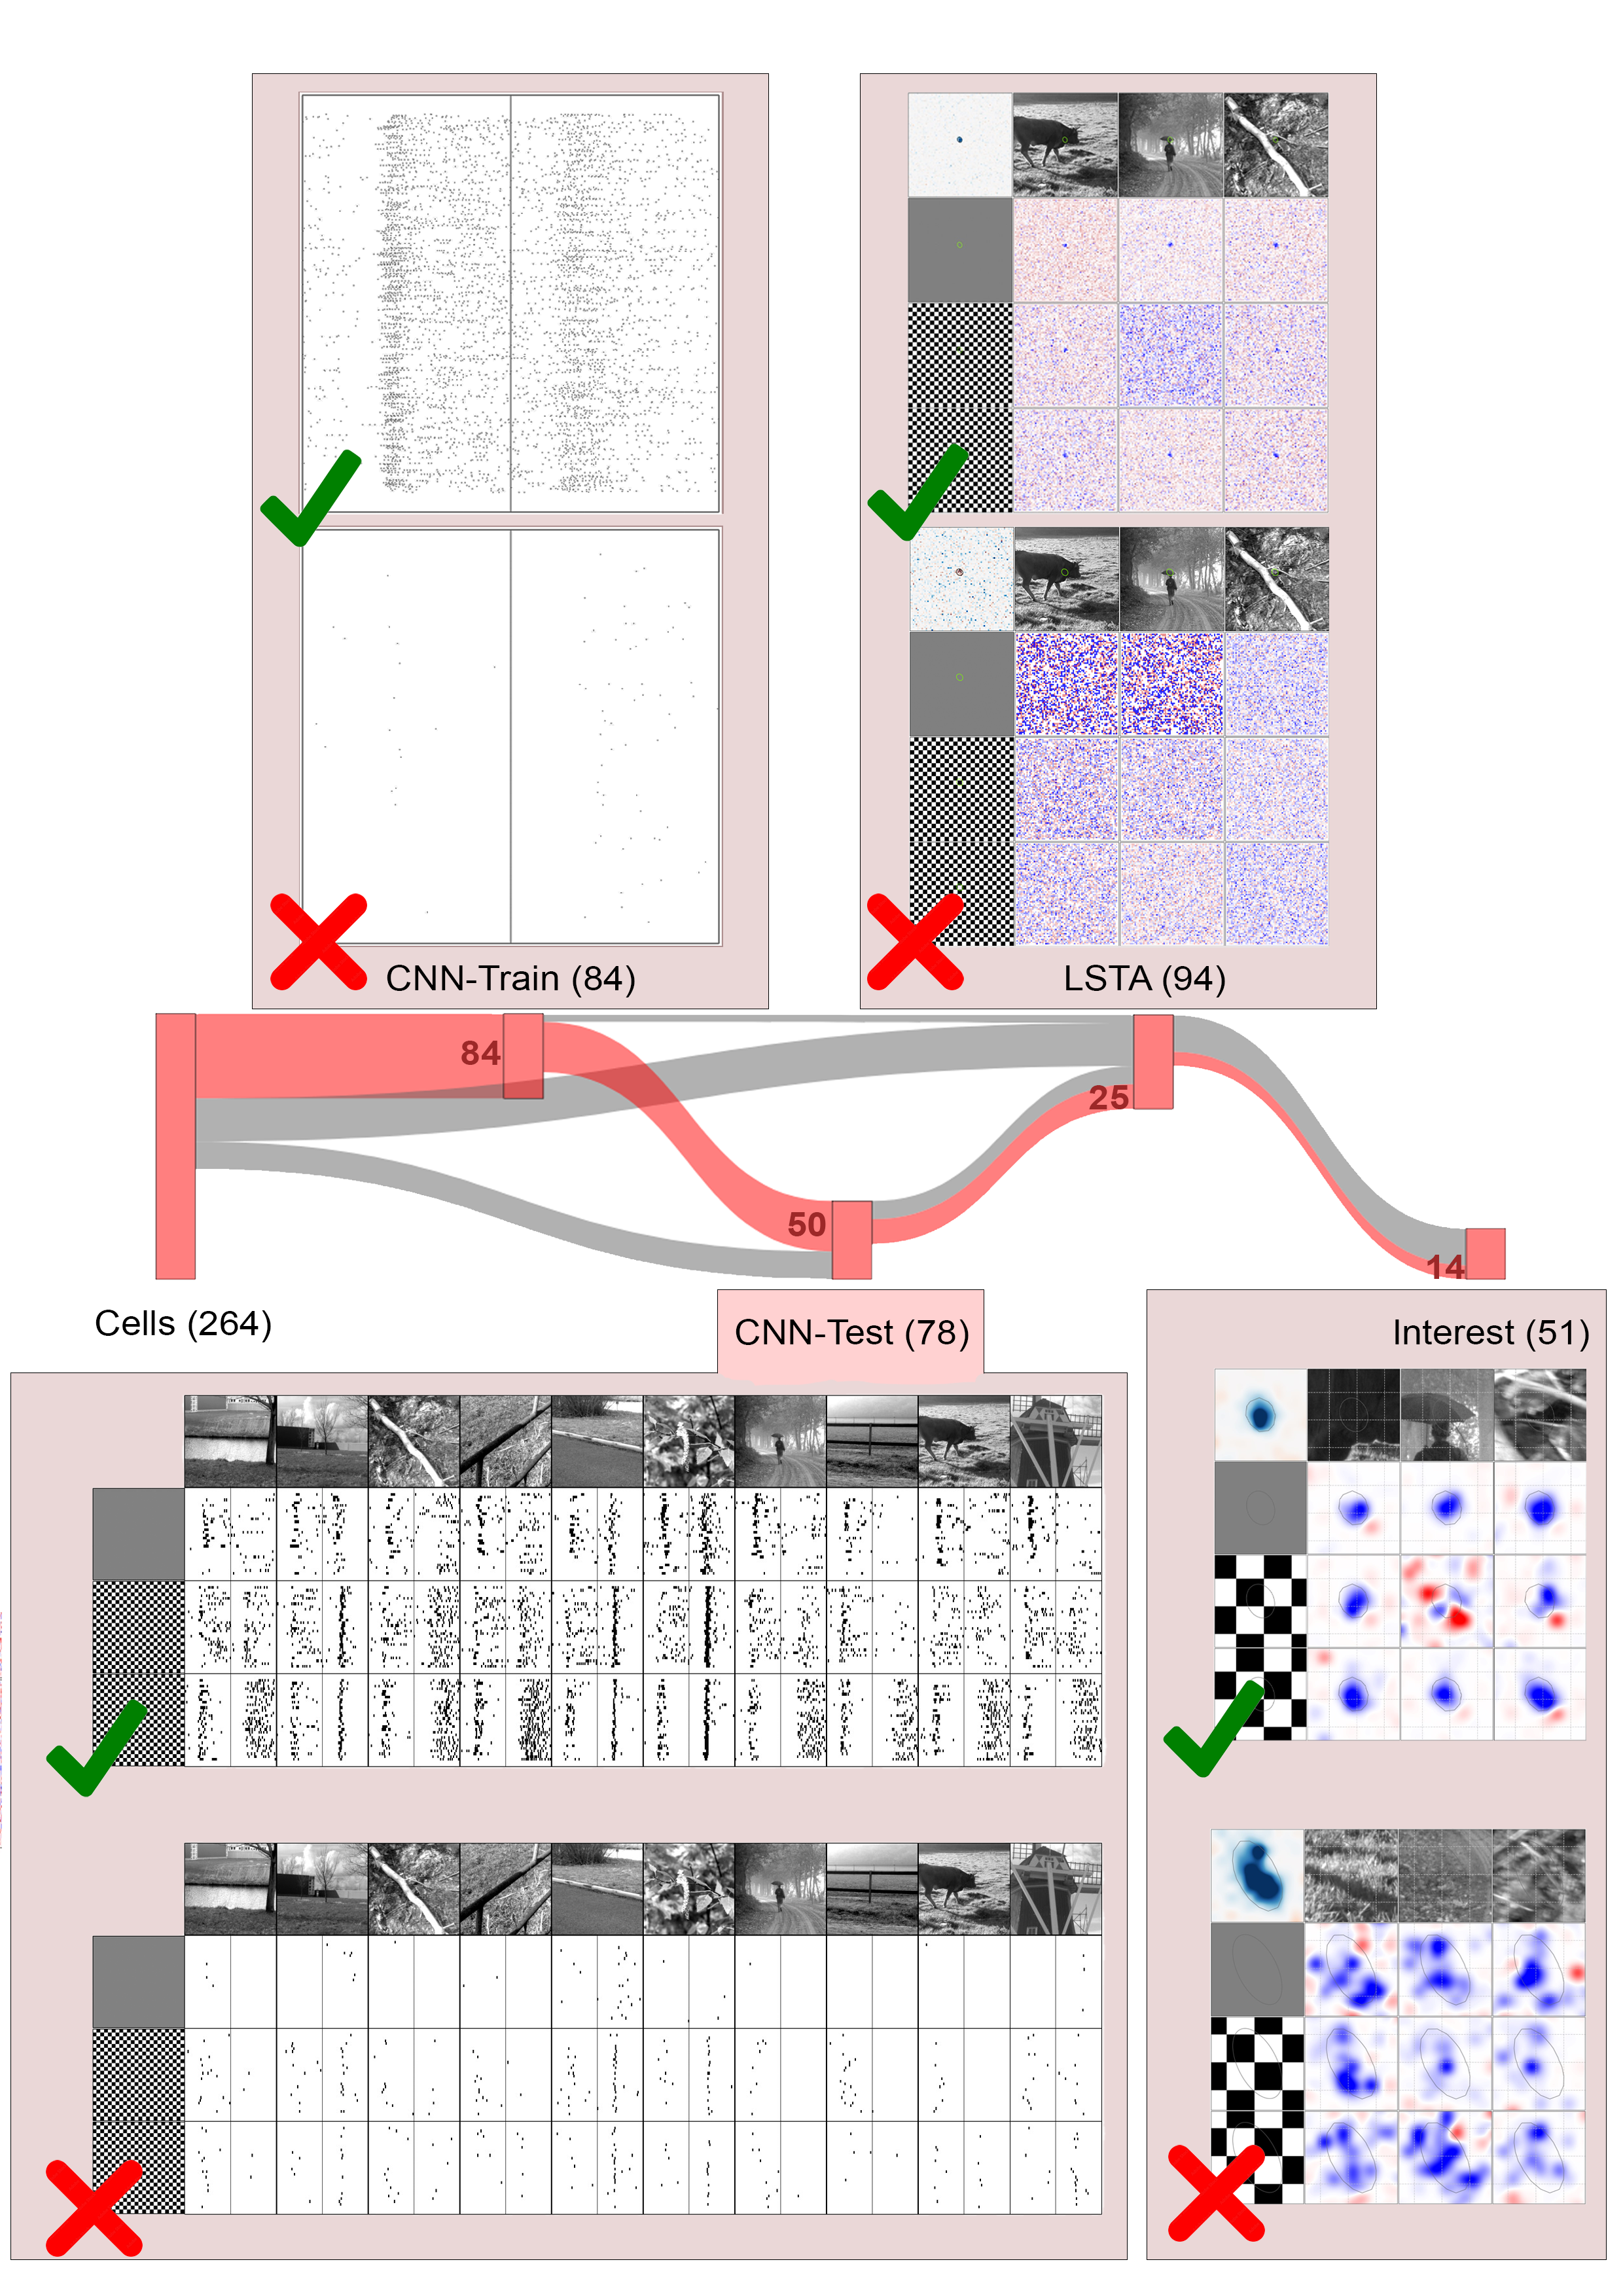
\includegraphics[width=0.8\textwidth]{pics/CellSelection.png}
    \caption{\textbf{Selecting cells suitable for the different degree of analysis.}}
    \label{fig:cell_selecion}
\end{figure}

% Graph idea : All type of rasters for one cell
% Bar chart representing the fading amount of data that can used for modeling

Blablable to share my programming skills to help and improve the data pipeline
of
the
laboratory.

% Models : Put the emphasis on the balance between G.C. and data-driven models
% Also insist on the time component of the models
\textbf{Modeling.} This should be the main part of my internship and also the
most challenging. We are designing a dynamical model of the retinal fast
adaptation. In fact, we mostly look at the evolution of the response from an
image to another, meaning that the dynamic we observe only spans two points in
time. This reduction makes the model more realistic to study. Most of this job
can be summarized as model design, python programming, sensitivity analysis and
data fitting. By comparing how different modeling strategies reproduce the
observed LSTA in the data, we can gain insight on how fast adaptation to
natural scene is implemented in the retina.
%I think what is missing here is what question you want to answer with this. We should discuss this more. 

Our baseline model is the LNLN model of ganglion cell widely used in the
literature. Each neuron is encoded as a spatial linear filter chained with a
non-linearity (usually an activation linearity in the like of ReLU). A single
layer of subunit neurons, representing bipolar cells, converge into a single
modeled ganglion cell.	We would like to add temporal dynamics to this model,
either by adding a time dimension to the spatial liner filter of the cells or
by considering a gain control mechanism. This last mechanism consists in
scaling up or down the present output depending on past outputs (Figure
TO FIND~\cite{}).

\begin{figure}
    \centering
    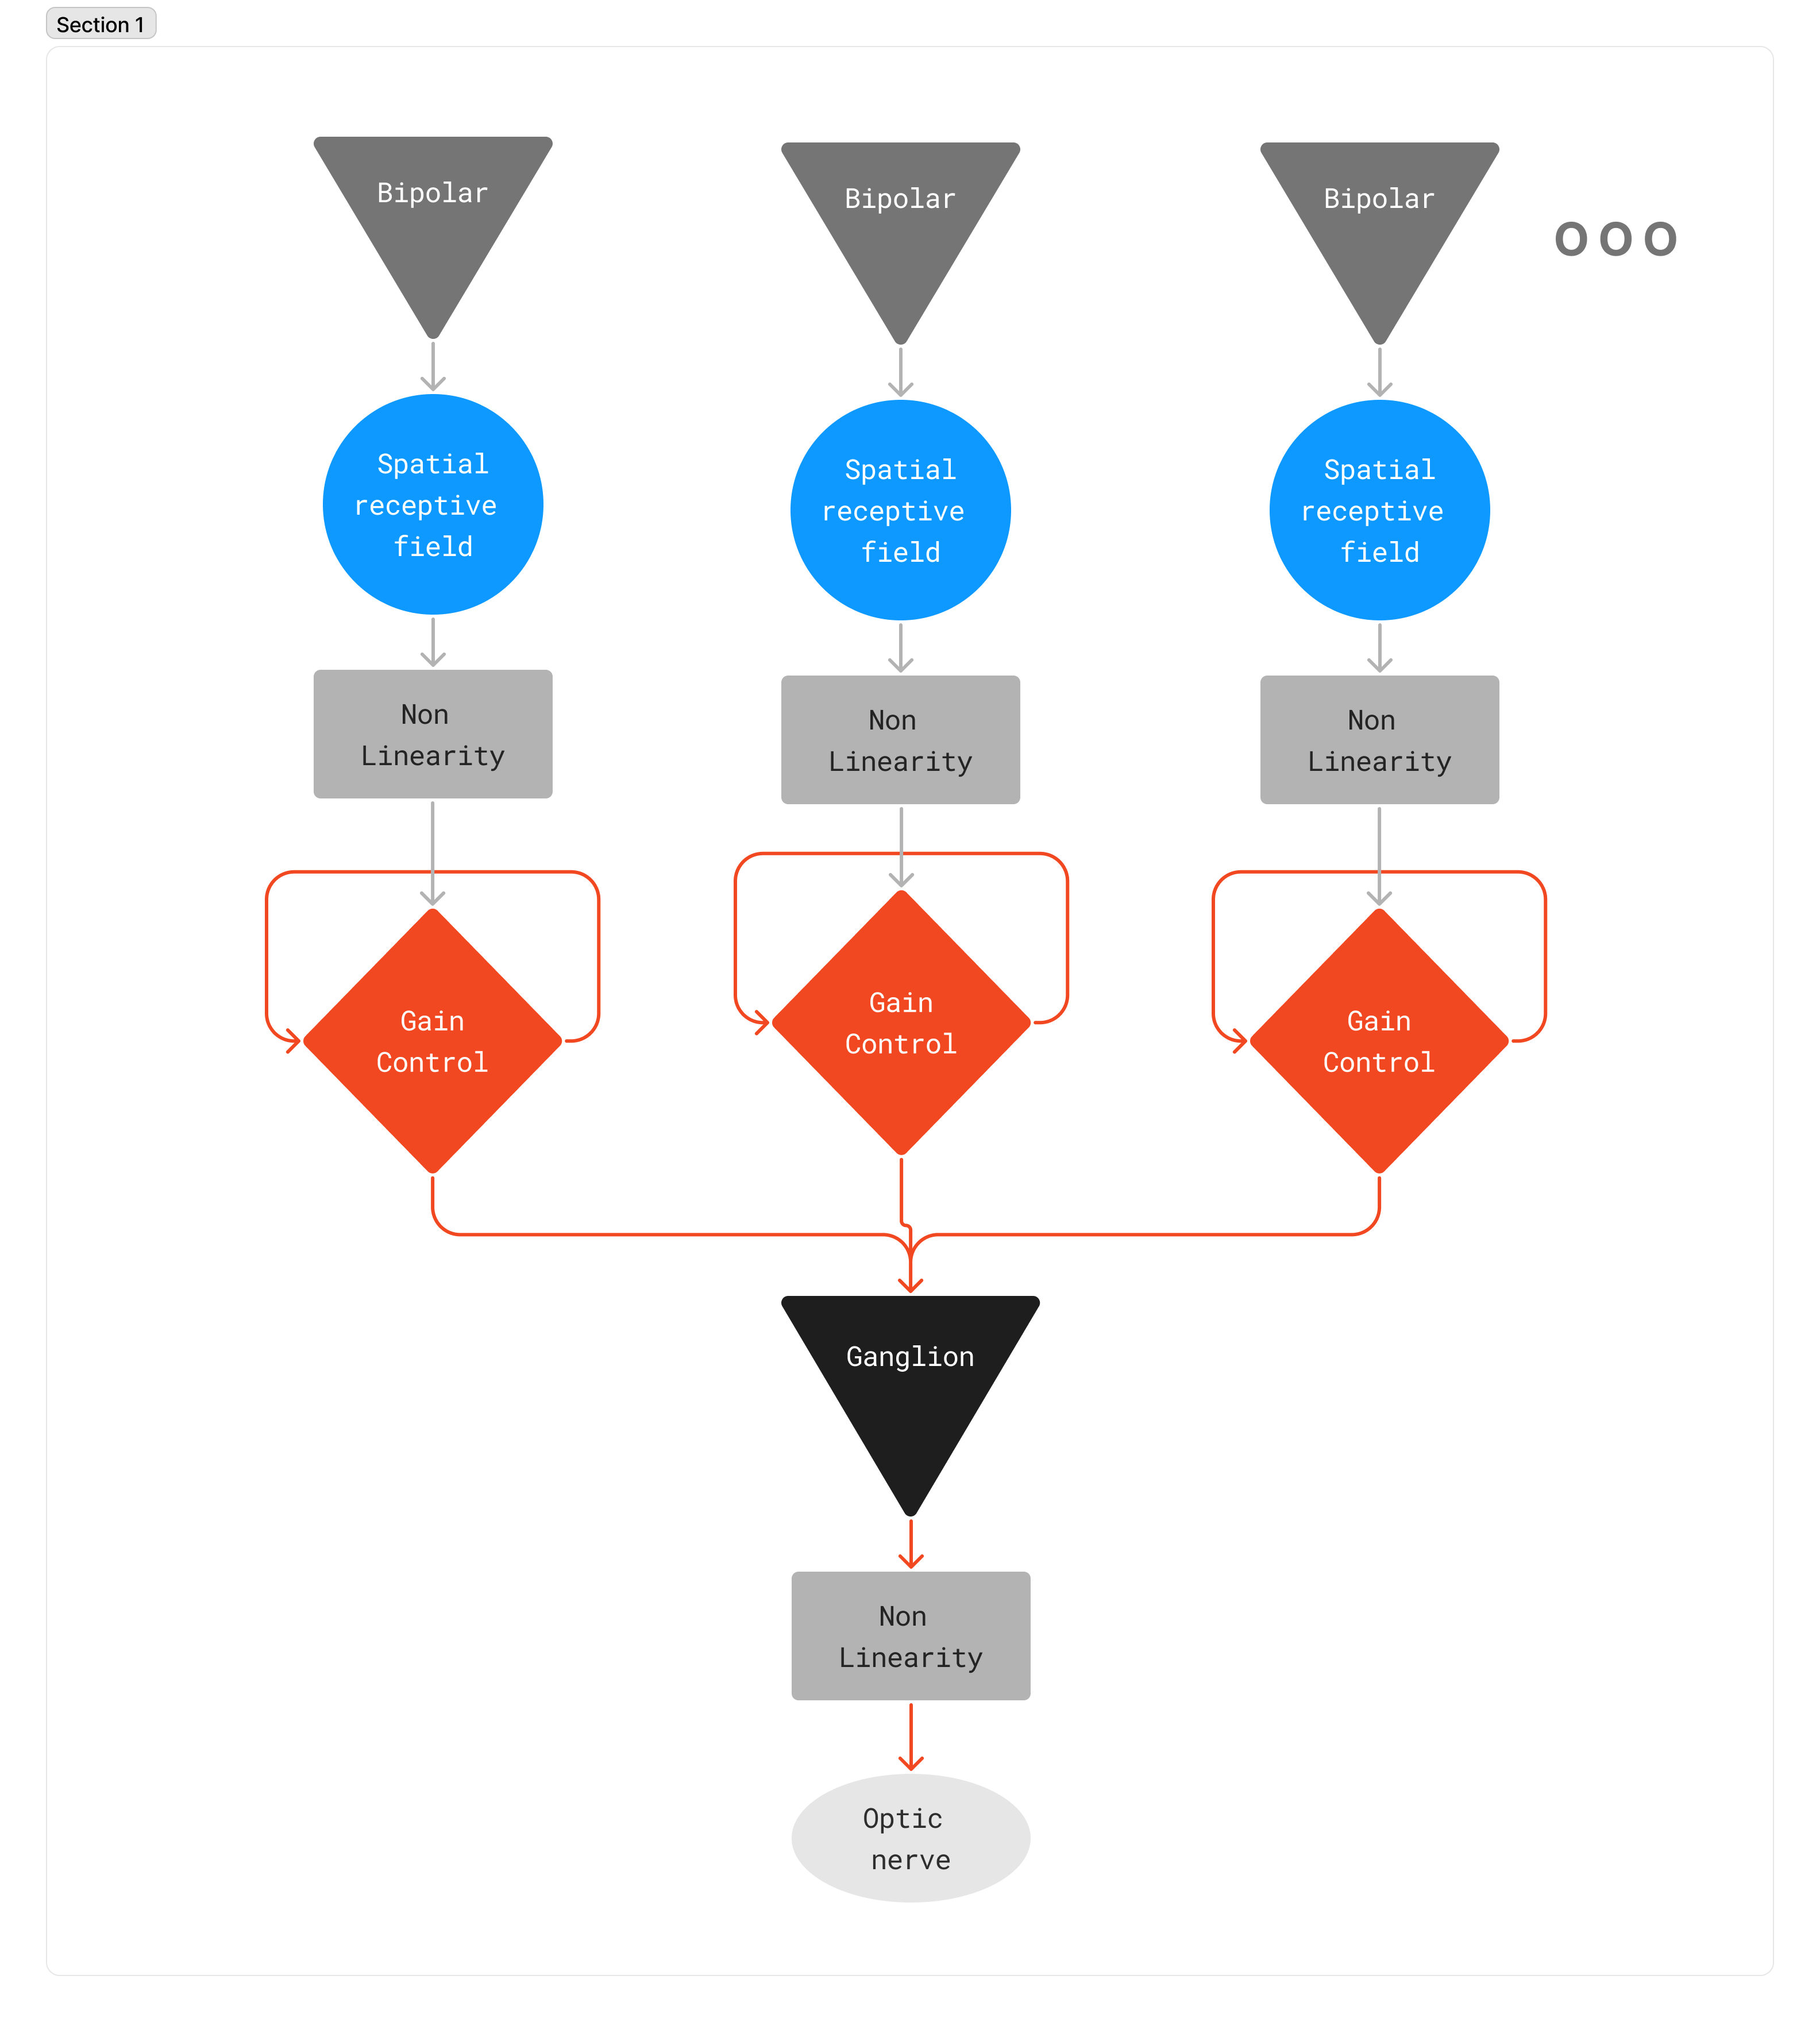
\includegraphics[scale = 0.2]{pics/GCModelDiagram.png}
    \caption{\textbf{Quick sketch of a gain control LNLN model.} Each bipolar
        cell is
        composed of a linear spatial filter that selectively responds to part
        of the scene,
        a non-linear activation function, and a gain control mechanism that
        scale its output
        depending on past events. They all converge into on bipolar cell
        (forming its receptive field)
        of which output is also modeled using a non-linear function.}
    \label{fig:LNLN}
\end{figure}
We will first study our models in a data agnostic manner and study its behavior
for different set of parameters. We will then fit it on our own experimental
data using an efficient optimization framework in python using strategies
developed in the field of machine learning.

In order to infer the non-linearities of the model, we will use a deepnet framework, optimized using the pytorch library.
In practice, we use a model that differ slightly from the LNLN model \ref*{label}.

\begin{figure}[h]
    \centering
    \includegraphics[width=0.8\textwidth]{pics/}
    \caption{\textbf{From anatomy to functional modeling.} In standard LN
        models,
        photoreceptors are considered purely linear and simply mapped to each
        pixel of
        the visual input. Bipolar cells tile the input space. They are modeled
        as a
        spatial linear filer, a difference of Gaussian defining a excitatory
        center and
        inhibitory surround, a biphasic linear temporal filter and a
        non-linearity.
        Ganglion cell pull and average the signal from all the bipolar cells in
        their
        receptive field, and spike selectively depending on their
        non-linearity. Notice the simplicity of LNLN model compared to the
        anatomical
        description of the retina.}
    \label{fig:retina_structure}
\end{figure}